\documentclass[border=4pt]{standalone}
\usepackage{amsmath,amssymb,tikz}
\usetikzlibrary{arrows.meta,calc}
\definecolor{figB}{RGB}{31,90,166}\definecolor{figR}{RGB}{176,48,48}\definecolor{figG}{RGB}{46,125,50}\definecolor{figO}{RGB}{214,120,20}
\begin{document}
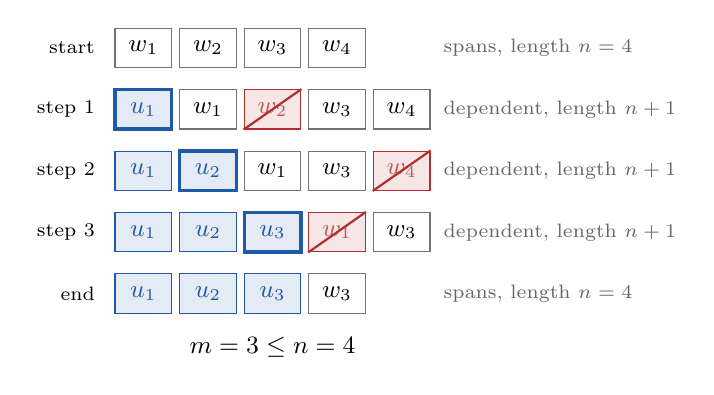
\begin{tikzpicture}[x=0.82cm,y=0.78cm,
  box/.style={draw=black!55,minimum width=0.72cm,minimum height=0.5cm,inner sep=0pt,font=\small},
  ubox/.style={box,draw=figB,fill=figB!12,text=figB},
  newu/.style={ubox,very thick},
  gone/.style={box,draw=figR,fill=figR!12,text=figR!80,
     append after command={(\tikzlastnode.south west) edge[figR,thick] (\tikzlastnode.north east)}}]
\def\row#1#2{\node[font=\scriptsize,anchor=east] at (-0.6,#1) {#2};}
\row{0}{start}
\node[box] at (0,0){$w_1$}; \node[box] at (1,0){$w_2$}; \node[box] at (2,0){$w_3$}; \node[box] at (3,0){$w_4$};
\node[font=\scriptsize,anchor=west,black!60] at (4.5,0) {spans, length $n=4$};
\row{-1}{step 1}
\node[newu] at (0,-1){$u_1$}; \node[box] at (1,-1){$w_1$}; \node[gone] at (2,-1){$w_2$}; \node[box] at (3,-1){$w_3$}; \node[box] at (4,-1){$w_4$};
\row{-2}{step 2}
\node[ubox] at (0,-2){$u_1$}; \node[newu] at (1,-2){$u_2$}; \node[box] at (2,-2){$w_1$}; \node[box] at (3,-2){$w_3$}; \node[gone] at (4,-2){$w_4$};
\row{-3}{step 3}
\node[ubox] at (0,-3){$u_1$}; \node[ubox] at (1,-3){$u_2$}; \node[newu] at (2,-3){$u_3$}; \node[gone] at (3,-3){$w_1$}; \node[box] at (4,-3){$w_3$};
\row{-4}{end}
\node[ubox] at (0,-4){$u_1$}; \node[ubox] at (1,-4){$u_2$}; \node[ubox] at (2,-4){$u_3$}; \node[box] at (3,-4){$w_3$};
\node[font=\scriptsize,anchor=west,black!60] at (4.5,-4) {spans, length $n=4$};
\foreach \y in {-1,-2,-3} \node[font=\scriptsize,anchor=west,black!60] at (4.5,\y) {dependent, length $n+1$};
\node[font=\small,anchor=north] at (2,-4.55) {$m=3\le n=4$};
\end{tikzpicture}
\end{document}
